
\tikzset{every picture/.style={line width=0.75pt}} %set default line width to 0.75pt        

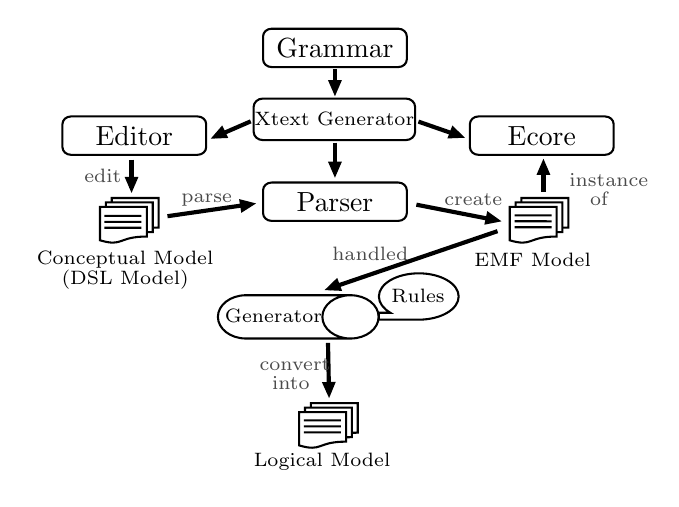
\begin{tikzpicture}[x=0.50pt,y=0.45pt,yscale=-1,xscale=1]
%uncomment if require: \path (0,465); %set diagram left start at 0, and has height of 465

%Rounded Rect [id:dp8080613887465731] 
\draw  [fill={rgb, 255:red, 255; green, 255; blue, 255 }  ,fill opacity=1 ] (166.24,24.37) .. controls (166.24,20.97) and (169,18.21) .. (172.4,18.21) -- (263.96,18.21) .. controls (267.36,18.21) and (270.11,20.97) .. (270.11,24.37) -- (270.11,42.84) .. controls (270.11,46.24) and (267.36,49) .. (263.96,49) -- (172.4,49) .. controls (169,49) and (166.24,46.24) .. (166.24,42.84) -- cycle ;
%Rounded Rect [id:dp23877247410758984] 
\draw  [fill={rgb, 255:red, 255; green, 255; blue, 255 }  ,fill opacity=1 ][line width=0.75]  (21.24,94.82) .. controls (21.24,91.42) and (24,88.66) .. (27.4,88.66) -- (118.95,88.66) .. controls (122.36,88.66) and (125.11,91.42) .. (125.11,94.82) -- (125.11,113.3) .. controls (125.11,116.7) and (122.36,119.46) .. (118.95,119.46) -- (27.4,119.46) .. controls (24,119.46) and (21.24,116.7) .. (21.24,113.3) -- cycle ;
%Flowchart: Multidocument [id:dp49717070559395604] 
\draw  [fill={rgb, 255:red, 255; green, 255; blue, 255 }  ,fill opacity=1 ] (56.88,154.12) -- (90.75,154.12) -- (90.75,177.89) .. controls (69.58,177.89) and (73.82,186.46) .. (56.88,180.91) -- cycle ; \draw  [fill={rgb, 255:red, 255; green, 255; blue, 255 }  ,fill opacity=1 ] (52.64,157.72) -- (86.52,157.72) -- (86.52,181.49) .. controls (65.35,181.49) and (69.58,190.06) .. (52.64,184.52) -- cycle ; \draw  [fill={rgb, 255:red, 255; green, 255; blue, 255 }  ,fill opacity=1 ] (48.41,161.32) -- (82.28,161.32) -- (82.28,185.09) .. controls (61.11,185.09) and (65.35,193.66) .. (48.41,188.12) -- cycle ;
%Straight Lines [id:da5642847406466045] 
\draw [fill={rgb, 255:red, 255; green, 255; blue, 255 }  ,fill opacity=1 ]   (51.63,168.47) -- (78.34,168.5) ;
%Straight Lines [id:da9779186616916171] 
\draw [fill={rgb, 255:red, 255; green, 255; blue, 255 }  ,fill opacity=1 ]   (51.63,173.26) -- (78.34,173.28) ;
%Straight Lines [id:da8217185402464098] 
\draw [fill={rgb, 255:red, 255; green, 255; blue, 255 }  ,fill opacity=1 ]   (51.63,178.04) -- (78.34,178.06) ;

%Straight Lines [id:da27204357118531197] 
\draw [fill={rgb, 255:red, 255; green, 255; blue, 255 }  ,fill opacity=1 ][line width=1.5]    (71.18,123.3) -- (71.18,146.06) ;
\draw [shift={(71.18,150.06)}, rotate = 270] [fill={rgb, 255:red, 0; green, 0; blue, 0 }  ][line width=0.08]  [draw opacity=0] (11.61,-5.58) -- (0,0) -- (11.61,5.58) -- cycle    ;
%Rounded Rect [id:dp014713549076222021] 
\draw  [fill={rgb, 255:red, 255; green, 255; blue, 255 }  ,fill opacity=1 ] (159.43,80.98) .. controls (159.43,77.3) and (162.41,74.31) .. (166.09,74.31) -- (269.45,74.31) .. controls (273.13,74.31) and (276.11,77.3) .. (276.11,80.98) -- (276.11,100.98) .. controls (276.11,104.66) and (273.13,107.65) .. (269.45,107.65) -- (166.09,107.65) .. controls (162.41,107.65) and (159.43,104.66) .. (159.43,100.98) -- cycle ;
%Rounded Rect [id:dp8159423215616721] 
\draw  [fill={rgb, 255:red, 255; green, 255; blue, 255 }  ,fill opacity=1 ] (315.72,94.82) .. controls (315.72,91.42) and (318.48,88.66) .. (321.88,88.66) -- (413.44,88.66) .. controls (416.84,88.66) and (419.59,91.42) .. (419.59,94.82) -- (419.59,113.3) .. controls (419.59,116.7) and (416.84,119.46) .. (413.44,119.46) -- (321.88,119.46) .. controls (318.48,119.46) and (315.72,116.7) .. (315.72,113.3) -- cycle ;
%Flowchart: Multidocument [id:dp814245162277164] 
\draw  [fill={rgb, 255:red, 255; green, 255; blue, 255 }  ,fill opacity=1 ] (352.96,154.12) -- (386.83,154.12) -- (386.83,177.89) .. controls (365.66,177.89) and (369.89,186.46) .. (352.96,180.91) -- cycle ; \draw  [fill={rgb, 255:red, 255; green, 255; blue, 255 }  ,fill opacity=1 ] (348.72,157.72) -- (382.6,157.72) -- (382.6,181.49) .. controls (361.43,181.49) and (365.66,190.06) .. (348.72,184.52) -- cycle ; \draw  [fill={rgb, 255:red, 255; green, 255; blue, 255 }  ,fill opacity=1 ] (344.49,161.32) -- (378.36,161.32) -- (378.36,185.09) .. controls (357.19,185.09) and (361.43,193.66) .. (344.49,188.12) -- cycle ;
%Straight Lines [id:da659202853659377] 
\draw [fill={rgb, 255:red, 255; green, 255; blue, 255 }  ,fill opacity=1 ]   (347.97,168.04) -- (374.69,168.06) ;
%Straight Lines [id:da8271632436642871] 
\draw [fill={rgb, 255:red, 255; green, 255; blue, 255 }  ,fill opacity=1 ]   (347.97,172.82) -- (374.69,172.85) ;
%Straight Lines [id:da22701123408508272] 
\draw [fill={rgb, 255:red, 255; green, 255; blue, 255 }  ,fill opacity=1 ]   (347.97,177.61) -- (374.69,177.63) ;

%Straight Lines [id:da6612735011438882] 
\draw [fill={rgb, 255:red, 255; green, 255; blue, 255 }  ,fill opacity=1 ][line width=1.5]    (368.86,126.65) -- (368.86,149.4) ;
\draw [shift={(368.86,122.65)}, rotate = 90] [fill={rgb, 255:red, 0; green, 0; blue, 0 }  ][line width=0.08]  [draw opacity=0] (11.61,-5.58) -- (0,0) -- (11.61,5.58) -- cycle    ;
%Rounded Rect [id:dp9641259565957541] 
\draw  [fill={rgb, 255:red, 255; green, 255; blue, 255 }  ,fill opacity=1 ] (166.24,147.89) .. controls (166.24,144.48) and (169,141.73) .. (172.4,141.73) -- (263.96,141.73) .. controls (267.36,141.73) and (270.11,144.48) .. (270.11,147.89) -- (270.11,166.36) .. controls (270.11,169.76) and (267.36,172.52) .. (263.96,172.52) -- (172.4,172.52) .. controls (169,172.52) and (166.24,169.76) .. (166.24,166.36) -- cycle ;
%Straight Lines [id:da4555835119587406] 
\draw [fill={rgb, 255:red, 255; green, 255; blue, 255 }  ,fill opacity=1 ][line width=1.5]    (218.18,50.89) -- (218.18,68.42) ;
\draw [shift={(218.18,72.42)}, rotate = 270] [fill={rgb, 255:red, 0; green, 0; blue, 0 }  ][line width=0.08]  [draw opacity=0] (11.61,-5.58) -- (0,0) -- (11.61,5.58) -- cycle    ;
%Straight Lines [id:da2586670416419199] 
\draw [fill={rgb, 255:red, 255; green, 255; blue, 255 }  ,fill opacity=1 ][line width=1.5]    (218.18,109.78) -- (218.18,133.88) ;
\draw [shift={(218.18,137.88)}, rotate = 270] [fill={rgb, 255:red, 0; green, 0; blue, 0 }  ][line width=0.08]  [draw opacity=0] (11.61,-5.58) -- (0,0) -- (11.61,5.58) -- cycle    ;
%Straight Lines [id:da2552674310073062] 
\draw [fill={rgb, 255:red, 255; green, 255; blue, 255 }  ,fill opacity=1 ][line width=1.5]    (157.32,92.59) -- (132.04,104.77) ;
\draw [shift={(128.43,106.51)}, rotate = 334.28] [fill={rgb, 255:red, 0; green, 0; blue, 0 }  ][line width=0.08]  [draw opacity=0] (11.61,-5.58) -- (0,0) -- (11.61,5.58) -- cycle    ;
%Straight Lines [id:da29550662771480396] 
\draw [fill={rgb, 255:red, 255; green, 255; blue, 255 }  ,fill opacity=1 ][line width=1.5]    (308.34,104.31) -- (278.52,92.81) ;
\draw [shift={(312.07,105.76)}, rotate = 201.11] [fill={rgb, 255:red, 0; green, 0; blue, 0 }  ][line width=0.08]  [draw opacity=0] (11.61,-5.58) -- (0,0) -- (11.61,5.58) -- cycle    ;
%Straight Lines [id:da3280771928101003] 
\draw [fill={rgb, 255:red, 255; green, 255; blue, 255 }  ,fill opacity=1 ][line width=1.5]    (97.15,168.77) -- (157.22,159.13) ;
\draw [shift={(161.17,158.5)}, rotate = 530.89] [fill={rgb, 255:red, 0; green, 0; blue, 0 }  ][line width=0.08]  [draw opacity=0] (11.61,-5.58) -- (0,0) -- (11.61,5.58) -- cycle    ;
%Straight Lines [id:da9478402467031726] 
\draw [fill={rgb, 255:red, 255; green, 255; blue, 255 }  ,fill opacity=1 ][line width=1.5]    (277.03,159.51) -- (334.63,172.02) ;
\draw [shift={(338.54,172.87)}, rotate = 192.26] [fill={rgb, 255:red, 0; green, 0; blue, 0 }  ][line width=0.08]  [draw opacity=0] (11.61,-5.58) -- (0,0) -- (11.61,5.58) -- cycle    ;
%Flowchart: Direct Access Storage [id:dp7657317583515377] 
\draw  [fill={rgb, 255:red, 255; green, 255; blue, 255 }  ,fill opacity=1 ] (229.43,266.99) -- (153.92,266.99) .. controls (142.69,266.99) and (133.59,259.2) .. (133.59,249.6) .. controls (133.59,240) and (142.69,232.21) .. (153.92,232.21) -- (229.43,232.21)(249.75,249.6) .. controls (249.75,259.2) and (240.65,266.99) .. (229.43,266.99) .. controls (218.2,266.99) and (209.1,259.2) .. (209.1,249.6) .. controls (209.1,240) and (218.2,232.21) .. (229.43,232.21) .. controls (240.65,232.21) and (249.75,240) .. (249.75,249.6) ;
%Straight Lines [id:da100480350897858] 
\draw [fill={rgb, 255:red, 255; green, 255; blue, 255 }  ,fill opacity=1 ][line width=1.5]    (335.65,180.79) -- (214.46,226.67) ;
\draw [shift={(210.72,228.08)}, rotate = 339.27] [fill={rgb, 255:red, 0; green, 0; blue, 0 }  ][line width=0.08]  [draw opacity=0] (11.61,-5.58) -- (0,0) -- (11.61,5.58) -- cycle    ;
%Flowchart: Multidocument [id:dp5253239734010293] 
\draw  [fill={rgb, 255:red, 255; green, 255; blue, 255 }  ,fill opacity=1 ] (200.79,318.82) -- (234.67,318.82) -- (234.67,342.59) .. controls (213.5,342.59) and (217.73,351.16) .. (200.79,345.61) -- cycle ; \draw  [fill={rgb, 255:red, 255; green, 255; blue, 255 }  ,fill opacity=1 ] (196.56,322.42) -- (230.44,322.42) -- (230.44,346.19) .. controls (209.26,346.19) and (213.5,354.76) .. (196.56,349.21) -- cycle ; \draw  [fill={rgb, 255:red, 255; green, 255; blue, 255 }  ,fill opacity=1 ] (192.32,326.02) -- (226.2,326.02) -- (226.2,349.79) .. controls (205.03,349.79) and (209.26,358.36) .. (192.32,352.81) -- cycle ;
%Straight Lines [id:da29635223798470123] 
\draw [fill={rgb, 255:red, 255; green, 255; blue, 255 }  ,fill opacity=1 ]   (195.81,332.74) -- (222.53,332.76) ;
%Straight Lines [id:da45709195099870326] 
\draw [fill={rgb, 255:red, 255; green, 255; blue, 255 }  ,fill opacity=1 ]   (195.81,337.52) -- (222.53,337.54) ;
%Straight Lines [id:da9397926099052756] 
\draw [fill={rgb, 255:red, 255; green, 255; blue, 255 }  ,fill opacity=1 ]   (195.81,342.31) -- (222.53,342.33) ;


%Straight Lines [id:da10826901476686546] 
\draw [fill={rgb, 255:red, 255; green, 255; blue, 255 }  ,fill opacity=1 ][line width=1.5]    (213.16,270.55) -- (213.89,310.78) ;
\draw [shift={(213.96,314.78)}, rotate = 268.97] [fill={rgb, 255:red, 0; green, 0; blue, 0 }  ][line width=0.08]  [draw opacity=0] (11.61,-5.58) -- (0,0) -- (11.61,5.58) -- cycle    ;
%Flowchart: Sequential Access Storage [id:dp3007368871754543] 
\draw  [fill={rgb, 255:red, 255; green, 255; blue, 255 }  ,fill opacity=1 ] (307.6,233.24) .. controls (307.6,222.96) and (294.69,214.63) .. (278.76,214.63) .. controls (262.84,214.63) and (249.93,222.96) .. (249.93,233.24) .. controls (249.93,238.31) and (253.07,242.9) .. (258.17,246.26) -- (249.93,246.26) -- (249.93,251.84) -- (278.76,251.84) .. controls (294.69,251.84) and (307.6,243.51) .. (307.6,233.24) -- cycle ;

% Text Node
\draw (73.18,104.06) node   [align=left] {Editor};
% Text Node
\draw (367.66,104.06) node   [align=left] {Ecore};
% Text Node
\draw (218.18,157.12) node   [align=left] {Parser};
% Text Node
\draw (218.18,33.6) node  [font=\normalsize] [align=left] {Grammar};
% Text Node
\draw (66.54,203.99) node   [align=left] {{\scriptsize Conceptual Model}};
% Text Node
\draw (361.03,203.99) node   [align=left] {{\scriptsize EMF Model}};
% Text Node
\draw (173.76,249.14) node  [font=\footnotesize] [align=left] {\begin{minipage}[lt]{39.427624pt}\setlength\topsep{0pt}
\begin{center}
{\scriptsize Generator}
\end{center}

\end{minipage}};
% Text Node
\draw (208.86,365.69) node   [align=left] {{\scriptsize Logical Model}};
% Text Node
\draw (278.24,232.37) node  [font=\scriptsize] [align=left] {\begin{minipage}[lt]{20.957804000000003pt}\setlength\topsep{0pt}
\begin{center}
Rules
\end{center}

\end{minipage}};
% Text Node
\draw (34.8,128.16) node [anchor=north west][inner sep=0.75pt]  [font=\scriptsize,color={rgb, 255:red, 74; green, 74; blue, 74 }  ,opacity=1 ] [align=left] {edit};
% Text Node
\draw (105,148.18) node [anchor=north west][inner sep=0.75pt]  [font=\scriptsize,color={rgb, 255:red, 74; green, 74; blue, 74 }  ,opacity=1 ] [align=left] {parse};
% Text Node
\draw (295,148.18) node [anchor=north west][inner sep=0.75pt]  [font=\scriptsize,color={rgb, 255:red, 74; green, 74; blue, 74 }  ,opacity=1 ] [align=left] {create};
% Text Node
\draw (385.4,132.21) node [anchor=north west][inner sep=0.75pt]  [font=\scriptsize,color={rgb, 255:red, 74; green, 74; blue, 74 }  ,opacity=1 ] [align=left] {instance};
% Text Node
\draw (214,190.69) node [anchor=north west][inner sep=0.75pt]  [font=\scriptsize,color={rgb, 255:red, 74; green, 74; blue, 74 }  ,opacity=1 ] [align=left] {handled};
% Text Node
\draw (161.5,280.8) node [anchor=north west][inner sep=0.75pt]  [font=\scriptsize,color={rgb, 255:red, 74; green, 74; blue, 74 }  ,opacity=1 ] [align=left] {convert};
% Text Node
\draw (400.4,147.21) node [anchor=north west][inner sep=0.75pt]  [font=\scriptsize,color={rgb, 255:red, 74; green, 74; blue, 74 }  ,opacity=1 ] [align=left] {of};
% Text Node
\draw (217.77,90.98) node  [font=\scriptsize] [align=left] {Xtext Generator};
% Text Node
\draw (170.5,294.8) node [anchor=north west][inner sep=0.75pt]  [font=\scriptsize,color={rgb, 255:red, 74; green, 74; blue, 74 }  ,opacity=1 ] [align=left] {into};
% Text Node
\draw (66.54,219.99) node   [align=left] {{\scriptsize (DSL Model)}};


\end{tikzpicture}
